\documentclass[12pt,a4paper]{article}

\usepackage[utf8]{inputenc}
\usepackage[T2A]{fontenc}
\usepackage[russian]{babel}

\usepackage{graphicx}
\usepackage{booktabs}
\usepackage{amsmath}
\usepackage{float}
\usepackage{geometry}
\geometry{left=2.5cm,right=2.5cm,top=2cm,bottom=2cm}

\usepackage{hyperref}
\hypersetup{colorlinks=true,linkcolor=blue,urlcolor=blue}

\title{Компьютерная задача\\«Спектральный анализ сетевого трафика для обнаружения аномалий»\\Вариант 1}
\author{Бикметов Даниель Азатович}
\date{\today}

\begin{document}

\maketitle

\section{Цель работы}
Освоить дискретное преобразование Фурье для анализа временного ряда сетевого трафика и определить наличие аномальных частотных компонент.

\section{Исходные данные}
Дан файл \texttt{variant\_01.csv} с двумя колонками:
\begin{itemize}
    \item \texttt{index} — номер точки времени, \(0,\dots,499\);
    \item \texttt{traffic} — интенсивность трафика, пакетов в секунду.
\end{itemize}
Длина ряда \(N=500\).

\section{График временного ряда}
На рис.~\ref{fig:traffic} показан исходный временной ряд.

\begin{figure}[H]
    \centering
    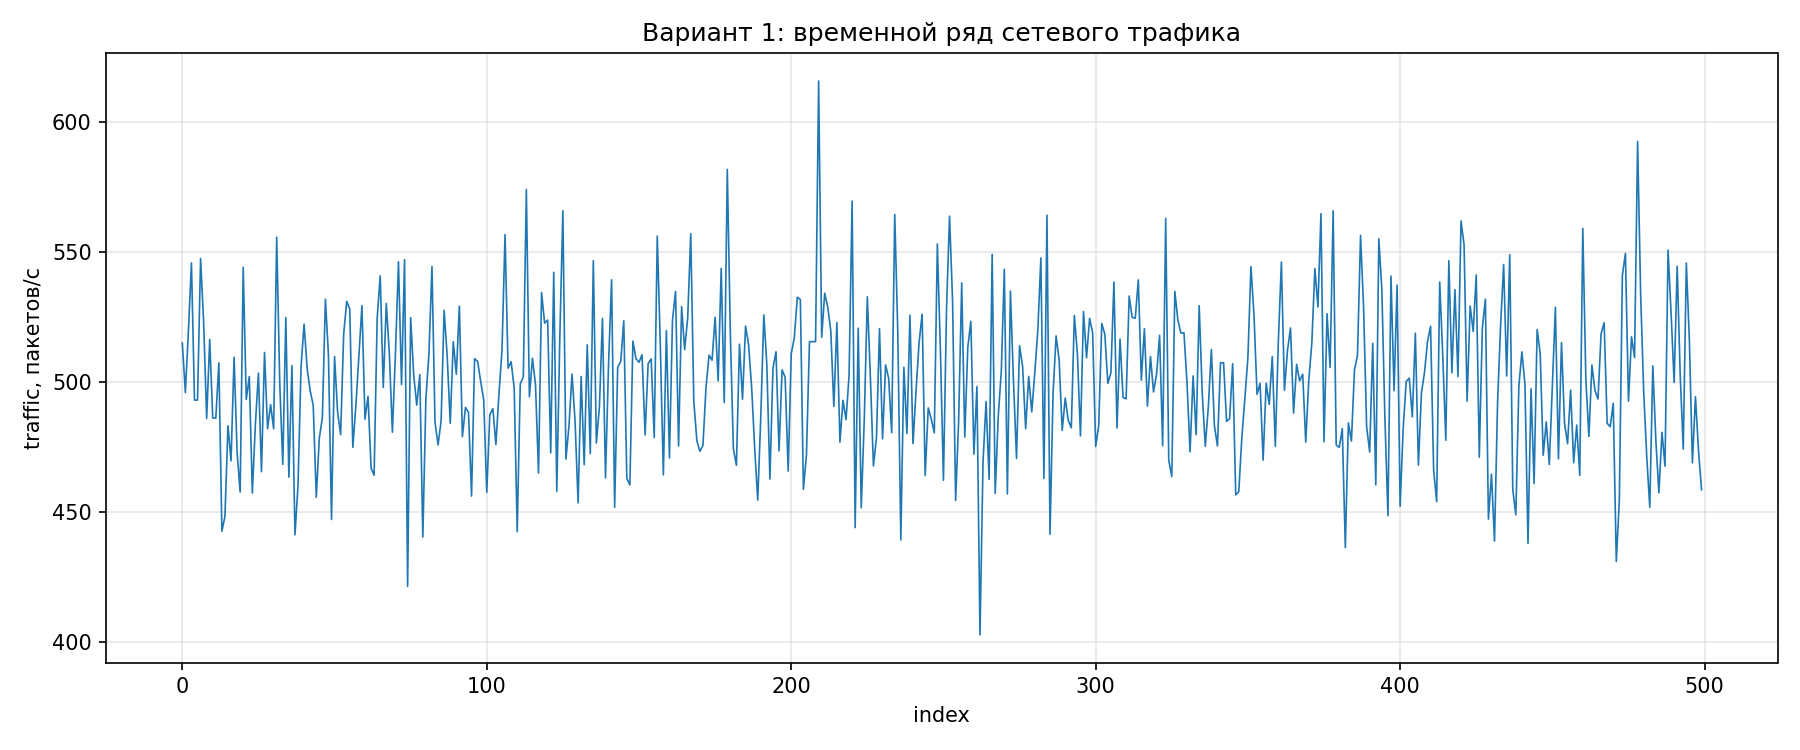
\includegraphics[width=0.95\textwidth]{01_traffic_series.png}
    \caption{Временной ряд интенсивности сетевого трафика для варианта 1}
    \label{fig:traffic}
\end{figure}

По графику видно, что трафик колеблется около среднего уровня примерно \(500\) пакетов/с. Выраженного монотонного тренда нет. Заметны отдельные выбросы, например:
\begin{itemize}
    \item \(index=209\): \(\approx 615.58\);
    \item \(index=179\): \(\approx 581.61\);
    \item \(index=113\): \(\approx 573.90\);
    \item \(index=262\): \(\approx 402.76\) — нижний выброс.
\end{itemize}
Окончательный вывод об аномальности делается по спектру.

\section{Вычисление коэффициентов Фурье}
Для \(k=0,1,\dots,50\) коэффициенты вычислялись вручную по формулам ДПФ без использования FFT:
\[
\frac{a_0}{2}=\frac{1}{N}\sum_{j=0}^{N-1}T(j),
\]
\[
a_k=\frac{2}{N}\sum_{j=0}^{N-1}T(j)\cos\left(\frac{2\pi kj}{N}\right),
\qquad
b_k=\frac{2}{N}\sum_{j=0}^{N-1}T(j)\sin\left(\frac{2\pi kj}{N}\right),
\]
\[
A_k=\sqrt{a_k^2+b_k^2}.
\]
Здесь \(N=500\). Результаты сохранены в файл \texttt{fourier\_coefficients\_variant\_01.csv}.

Средний уровень трафика:
\[
\frac{a_0}{2} \approx 500.21
\]

\section{Амплитудный спектр}
На рис.~\ref{fig:spectrum} приведён спектр \(A_k\) для \(k=1,\dots,50\).

\begin{figure}[H]
    \centering
    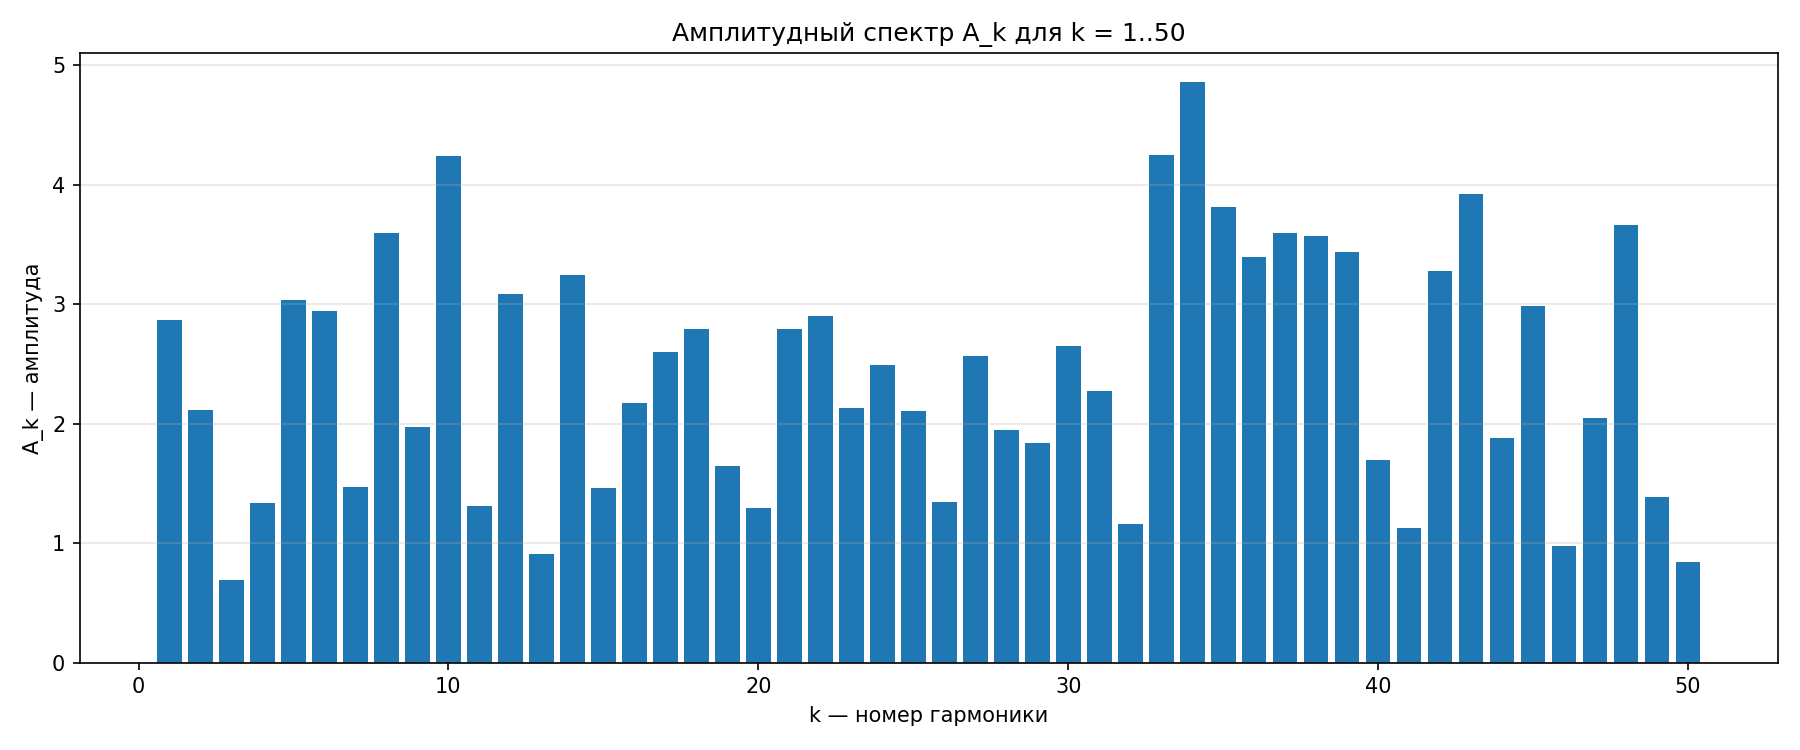
\includegraphics[width=0.95\textwidth]{02_spectrum.png}
    \caption{Амплитудный спектр \(A_k\) для \(k=1,\dots,50\)}
    \label{fig:spectrum}
\end{figure}

\begin{figure}[H]
    \centering
    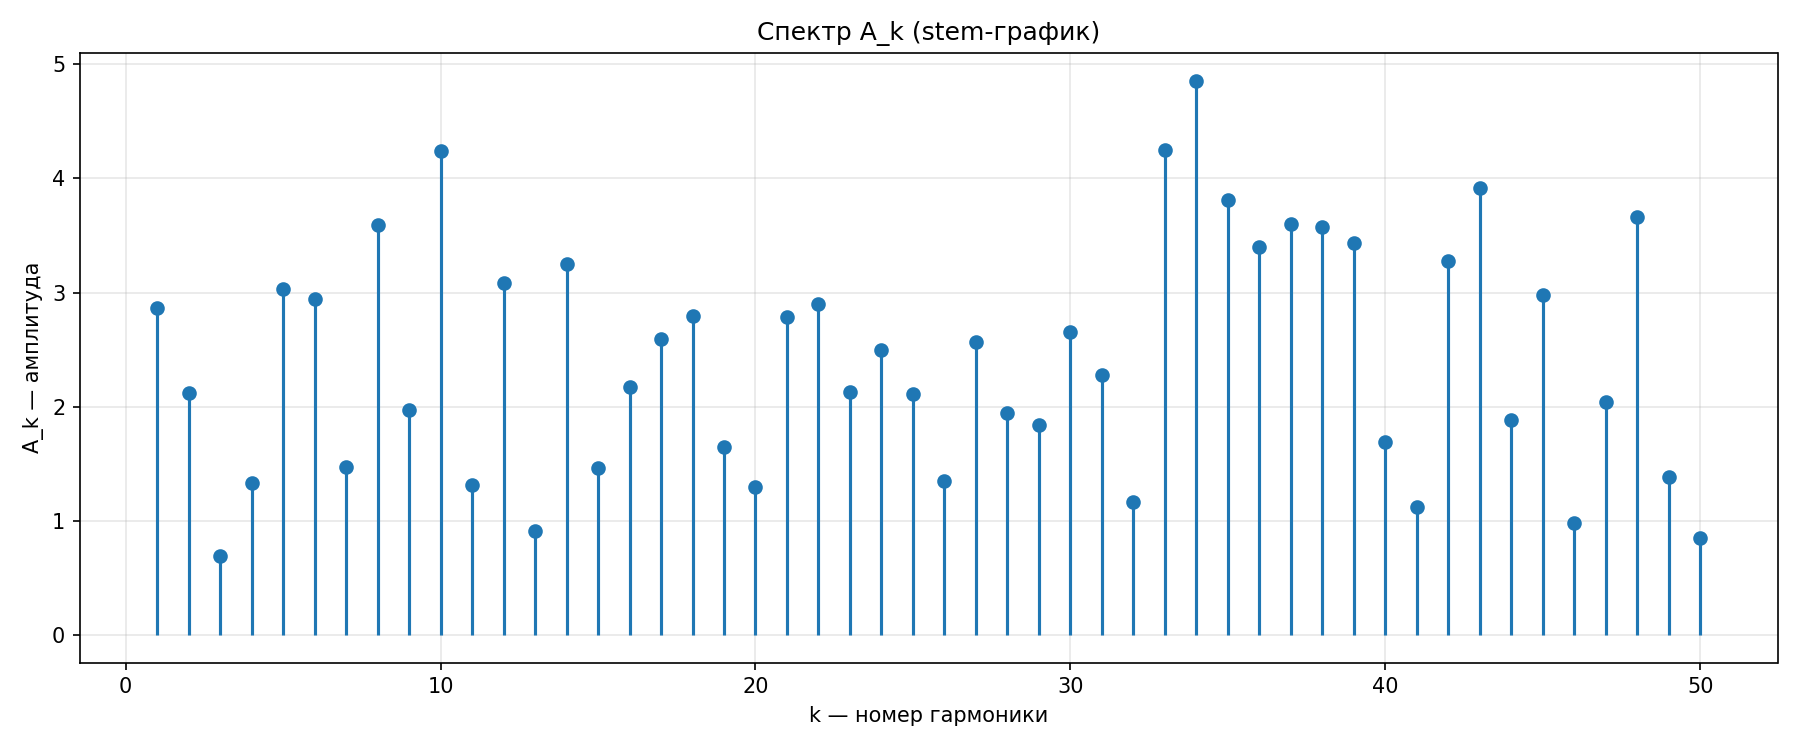
\includegraphics[width=0.95\textwidth]{04_spectrum_stem.png}
    \caption{Спектр \(A_k\) в виде stem-графика}
    \label{fig:spectrum_stem}
\end{figure}

Топ-10 гармоник по амплитуде:
\begin{table}[H]
    \centering
    \caption{Топ-10 гармоник по амплитуде \(A_k\)}
    \begin{tabular}{rr}
        \toprule
        \(k\) & \(A_k\) \\
        \midrule
        34 & 4.8571 \\
        33 & 4.2485 \\
        10 & 4.2436 \\
        43 & 3.9195 \\
        35 & 3.8138 \\
        48 & 3.6600 \\
        37 & 3.5984 \\
        8  & 3.5950 \\
        38 & 3.5744 \\
        39 & 3.4371 \\
        \bottomrule
    \end{tabular}
\end{table}

Средняя амплитуда и СКО по \(k=1,\dots,50\):
\[
\overline{A} \approx 2.47,
\qquad
\sigma_A \approx 1.35.
\]
Порог \(\overline{A}+3\sigma_A \approx 6.51\).

Гармоники, превышающие порог:
\begin{itemize}
    \item Гармоник, превышающих порог \(\overline{A}+3\sigma_A\), нет. Максимальная амплитуда (\(A_{34} \approx 4.86\)) значительно ниже порога.
\end{itemize}

\section{Определение аномалии}
Ответы на вопросы задания:
\begin{enumerate}
    \item Есть ли в спектре аномальные пики?
    
    Резко выделяющихся аномальных пиков не обнаружено. Хотя в спектре присутствуют локальные максимумы (например, на \(k=34\), \(k=33\) и \(k=10\)), их амплитуды не превышают статистический порог \(\overline{A}+3\sigma_A\), что говорит об их случайной природе или фоновом шуме, а не о целенаправленной атаке.
    
    \item На каких \(k\) они находятся?
    
    Наиболее заметные локальные пики находятся на \(k = 34\), \(33\) и \(10\). Однако аномальными в строгом смысле они не являются.
    
    \item Что это может означать?
    
    Признаков DDoS-атаки, ботнета, сканирования портов или скрытого канала по спектру не выявлено. Одиночные выбросы во временном ряду (index = 209, 179, 113, 262) не образуют устойчивой периодической компоненты и не дают характерного высокочастотного пика. Трафик в данном варианте близок к нормальному с шумом.
\end{enumerate}

\section{Тригонометрические приближения}
Построены приближения для \(K=2\) и \(K=20\):
\[
T_K(t)=\frac{a_0}{2}+\sum_{k=1}^{K}
\left(
a_k\cos\frac{2\pi kt}{N}+b_k\sin\frac{2\pi kt}{N}
\right).
\]
На рис.~\ref{fig:approx} показаны исходный ряд и оба приближения.

\begin{figure}[H]
    \centering
    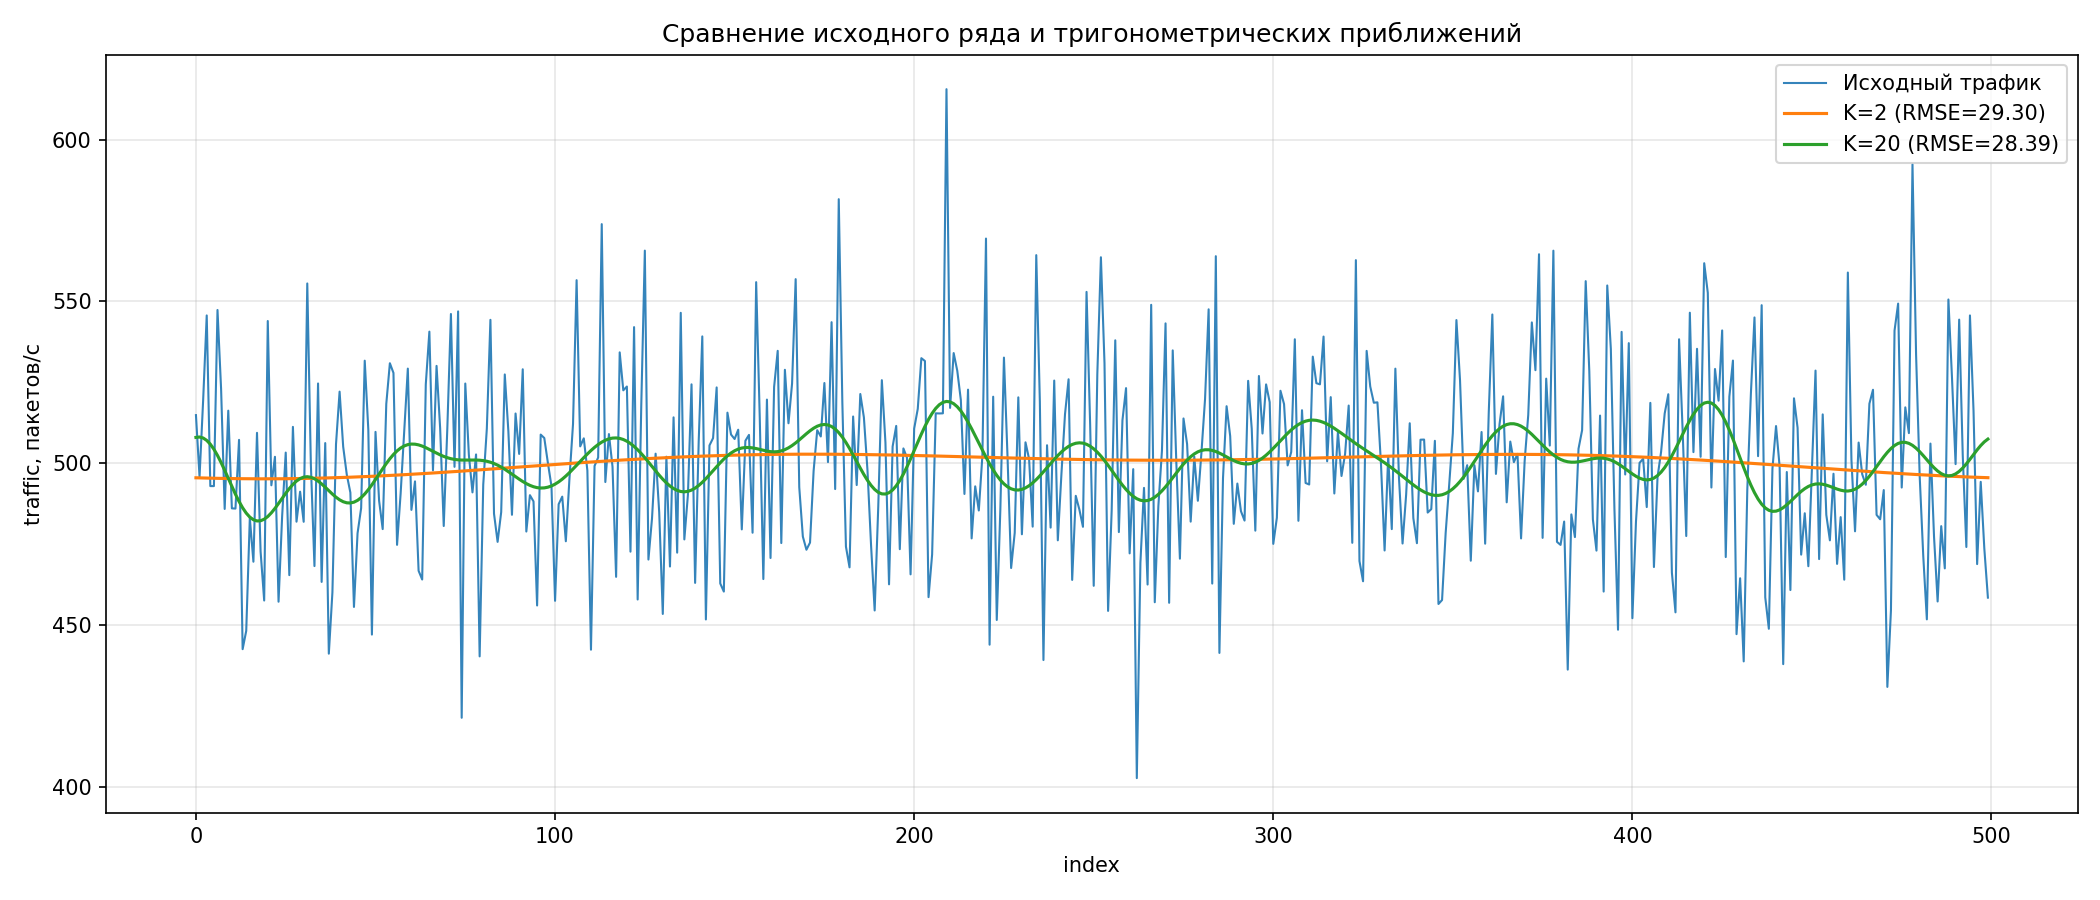
\includegraphics[width=0.98\textwidth]{03_approximations.png}
    \caption{Исходный ряд и приближения \(K=2\), \(K=20\)}
    \label{fig:approx}
\end{figure}

RMSE:
\[
\mathrm{RMSE}_{K=2} \approx 29.30,
\qquad
\mathrm{RMSE}_{K=20} \approx 28.39.
\]
Приближение \(K=20\) описывает данные немного лучше, чем \(K=2\), что подтверждается меньшим RMSE и визуально более близкой формой графика (появляются высокочастотные колебания, повторяющие контур сигнала). Однако даже \(K=20\) не улавливает одиночные резкие выбросы, так как они требуют значительно большего числа гармоник.

\section{Вывод}
В ходе работы построена спектральная модель временного ряда сетевого трафика для варианта 1. Коэффициенты Фурье вычислены вручную для \(k=0,\dots,50\). По спектру \(A_k\) аномальных частотных компонент, указывающих на DDoS-атаку или скрытый канал, не обнаружено. Наблюдаемые колебания и отдельные выбросы не образуют устойчивого пика на высокой частоте. Приближение \(K=20\) точнее описывает ряд, чем \(K=2\).

\end{document}
